% !TeX program = xelatex
\documentclass[a4paper,10pt]{article}

% ============================================================================
% ១. កញ្ចប់បណ្ណាល័យ និងការកំណត់ទំព័រ (Packages & Page Setup — តាមគំរូ ls_plan.tex)
% ============================================================================
\usepackage[a4paper, left=0.95cm, right=0.95cm, top=0.85cm, bottom=0.92cm, footskip=0.52cm]{geometry}
\usepackage{amsmath}
\usepackage{unicode-math}
\usepackage{fontspec}
\usepackage{longtable, array, multirow, colortbl}
\usepackage[table]{xcolor}
\usepackage{enumitem}
\usepackage{pifont}
\usepackage{fancyhdr}
\usepackage{tikz}
\usetikzlibrary{calc, arrows.meta, decorations.pathreplacing, patterns, positioning, babel}

\makeatletter
\let\@expl@@@mark@update@singlecol@structures@@\relax
\makeatother

% --- ប្រព័ន្ធស្វែងរកទីតាំងពុម្ពអក្សរស្វ័យប្រវត្តិ (Windows Local + Cloud Repo fonts/) ---
\providecommand{\NGSFindFonts}{%
  \IfFileExists{C:/Windows/Fonts/cambria.ttc}{%
    \def\NGSSysPath{C:/Windows/Fonts/}%
    \def\NGSUserPath{C:/Users/KIT/AppData/Local/Microsoft/Windows/Fonts/}%
  }{%
    \IfFileExists{./fonts/KhmerOSsiemreap.ttf}{\def\NGSSysPath{./fonts/}\def\NGSUserPath{./fonts/}}{%
    \IfFileExists{../fonts/KhmerOSsiemreap.ttf}{\def\NGSSysPath{../fonts/}\def\NGSUserPath{../fonts/}}{%
    \IfFileExists{../../fonts/KhmerOSsiemreap.ttf}{\def\NGSSysPath{../../fonts/}\def\NGSUserPath{../../fonts/}}{%
    \IfFileExists{../../../fonts/KhmerOSsiemreap.ttf}{\def\NGSSysPath{../../../fonts/}\def\NGSUserPath{../../../fonts/}}{%
    \IfFileExists{../../../../fonts/KhmerOSsiemreap.ttf}{\def\NGSSysPath{../../../../fonts/}\def\NGSUserPath{../../../../fonts/}}{%
    \IfFileExists{../../../../../fonts/KhmerOSsiemreap.ttf}{\def\NGSSysPath{../../../../../fonts/}\def\NGSUserPath{../../../../../fonts/}}{%
    \IfFileExists{../../../../../../fonts/KhmerOSsiemreap.ttf}{\def\NGSSysPath{../../../../../../fonts/}\def\NGSUserPath{../../../../../../fonts/}}{%
      \def\NGSSysPath{../../../../../../../fonts/}\def\NGSUserPath{../../../../../../../fonts/}%
    }}}}}}}%
  }%
}
\NGSFindFonts

% ============================================================================
% ២. កំណត់ពុម្ពអក្សរ (Fonts — តាមគំរូ ls_plan.tex)
% ============================================================================
\setmathfont[Path={\NGSSysPath}, FontIndex=1, Scale=1.02]{cambria.ttc}
\defaultfontfeatures{Ligatures=TeX}

\setmainfont[
  Path={\NGSUserPath},
  Extension=.ttf,
  Script=Khmer,
  BoldFont={KhmerOSsiemreap},
  BoldFeatures={FakeBold=1.8},
  ItalicFont={KhmerOSsiemreap},
  ItalicFeatures={FakeSlant=0.25},
  BoldItalicFont={KhmerOSsiemreap},
  BoldItalicFeatures={FakeBold=1.8, FakeSlant=0.25}
]{KhmerOSsiemreap}

\newfontfamily\muol[Path={\NGSUserPath}, Extension=.ttf, Script=Khmer]{KhmerOSmuollight}
\newfontfamily\Tacteing[Path={\NGSUserPath}, Extension=.TTF]{TACTENG}
\newfontfamily\TimesEn[Path={\NGSSysPath}, Extension=.ttf, BoldFont={timesbd}, ItalicFont={timesi}, BoldItalicFont={timesbi}]{times}
\newfontfamily\CalibriFont[Path={\NGSSysPath}, Extension=.ttf]{calibri}
\newfontfamily\CourierCirc[Path={\NGSSysPath}, Extension=.ttf]{cour}

\XeTeXlinebreaklocale "km"
\XeTeXlinebreakskip = 0pt plus 1pt minus 0.1pt

% ============================================================================
% ៣. ពណ៌ និងការតុបតែង (Colors & Styles)
% ============================================================================
\definecolor{stepbg}{HTML}{D9D9D9}
\definecolor{headgray}{HTML}{E6E6E6}
\definecolor{emphred}{HTML}{C00000}

\pagestyle{fancy}
\fancyhf{}
\renewcommand{\headrulewidth}{0pt}
\fancyfoot[R]{\CalibriFont\fontsize{9pt}{11pt}\selectfont\thepage}

\setlength{\parindent}{0pt}
\setlength{\parskip}{0pt}
\setlength{\tabcolsep}{4.5pt}
\setlength{\LTpre}{2pt}
\setlength{\LTpost}{2pt}

\newcolumntype{L}[1]{>{\raggedright\arraybackslash}p{#1}}
\newcolumntype{C}[1]{>{\centering\arraybackslash}p{#1}}

% ============================================================================
% ៤. ពាក្យបញ្ជាជំនួយ (Helper Macros)
% ============================================================================
\newcommand{\en}[1]{{\TimesEn #1}}
\newcommand{\enbf}[1]{{\TimesEn\bfseries #1}}
\newcommand{\khmflourish}{{\Tacteing\fontsize{15pt}{15pt}\selectfont 3}}
\newcommand{\wcirc}{{\CourierCirc\fontsize{9.5pt}{11pt}\selectfont o}}
\newcommand{\ditem}{{\fontsize{7.5pt}{10pt}\selectfont\ding{117}}\ }
\newcommand{\fiveE}[1]{\textcolor{emphred}{\CalibriFont\bfseries #1}}
\newcommand{\redsub}[1]{\textcolor{emphred}{#1}}
\newcommand{\timenote}[1]{\textcolor{emphred}{\textit{#1}}}
\newcommand{\stepheader}[1]{\multicolumn{3}{|c|}{\cellcolor{stepbg}\muol #1} \\ \hline}
\newcommand{\cfig}[1]{{\centering\vspace{3pt}#1\vspace{3pt}\par}}
\newcommand{\cnum}[1]{\mbox{\fontsize{10.5pt}{12pt}\selectfont\ding{\numexpr181+#1\relax}}}
\newcommand{\unit}[1]{\,\text{\en{#1}}}
\newcommand{\graybox}[1]{\colorbox{headgray}{\strut #1}}

% ============================================================================
% ៥. រូបភាព TikZ ស-ខ្មៅ សម្រាប់បង្រៀនលើក្ដារខៀន និងសន្លឹកកិច្ចការ (B&W Diagrams)
% ============================================================================

% ១. E1 Engage: អន្ទាក់ពាក្យ «ធំបំផុត» លើ PGCD(12, 18)
\newcommand{\figEngageDIVTwoFive}{%
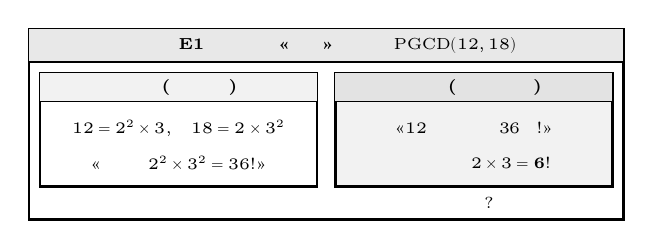
\begin{tikzpicture}[x=1cm, y=1cm, every node/.style={font=\fontsize{5.8pt}{7.7pt}\selectfont, text=black}]
  \draw[black, line width=0.9pt] (0,0) rectangle (7.55,2.42);
  \fill[gray!18] (0,2.00) rectangle (7.55,2.42);
  \draw[black, line width=0.6pt] (0,2.00) -- (7.55,2.00);
  \node at (3.775,2.21) {\textbf{បេសកកម្ម \en{E1}៖ អន្ទាក់ពាក្យ «ធំបំផុត» ក្នុងការរក $\operatorname{PGCD}(12, 18)$}};

  % Student A
  \draw[black, line width=0.8pt] (0.14,0.42) rectangle (3.66,1.86);
  \fill[gray!10] (0.14,1.50) rectangle (3.66,1.86);
  \draw[black, line width=0.5pt] (0.14,1.50) -- (3.66,1.50);
  \node at (1.90,1.68) {\textbf{សិស្ស ក (យកនិទស្សន្តធំ)}};
  \node at (1.90,1.16) {$12=2^2\times 3,\quad 18=2\times 3^2$};
  \node at (1.90,0.72) {«ធំបំផុតគឺ $2^2\times 3^2 = 36$!»};

  % Student B
  \draw[black, line width=0.95pt, fill=gray!10] (3.89,0.42) rectangle (7.41,1.86);
  \fill[gray!22] (3.89,1.50) rectangle (7.41,1.86);
  \draw[black, line width=0.55pt] (3.89,1.50) -- (7.41,1.50);
  \node at (5.65,1.68) {\textbf{សិស្ស ខ (ពិនិត្យភាពចែកដាច់)}};
  \node at (5.65,1.16) {«$12$ ចែកមិនដាច់នឹង $36$ ទេ!»};
  \node at (5.65,0.72) {យកនិទស្សន្តតូច៖ $2\times 3 = \mathbf{6}$!};

  \node at (3.775,0.21) {\textbf{សំណួរ៖} ហេតុអ្វីតួចែករួមធំបំផុតត្រូវជ្រើសយក\textbf{និទស្សន្តតូចជាងគេ}នៃកត្តាបឋមរួម?};
\end{tikzpicture}}

% ២. E2 Explore: ប្រអប់ជួរឈរកត្តាបឋម ទំ.២១ សម្រាប់ PGCD(30,36) និង PGCD(60,180,210)
\newcommand{\figPrimeColsDIVTwoFive}{%
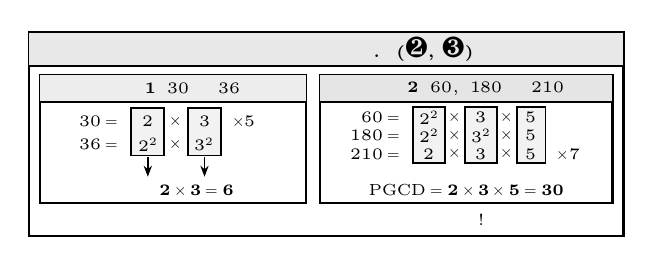
\begin{tikzpicture}[x=1cm, y=1cm, every node/.style={font=\fontsize{5.8pt}{7.6pt}\selectfont, text=black}]
  \draw[black, line width=0.9pt] (0,0) rectangle (7.55,2.58);
  \fill[gray!18] (0,2.16) rectangle (7.55,2.58);
  \draw[black, line width=0.6pt] (0,2.16) -- (7.55,2.16);
  \node at (3.775,2.37) {\textbf{តារាងតម្រឹមជួរឈរកត្តាបឋមរួម តាមសៀវភៅគោល ទំ.២១ (\cnum{2}, \cnum{3})}};

  % Left: 30 and 36
  \draw[black, line width=0.8pt] (0.14,0.42) rectangle (3.52,2.04);
  \fill[gray!14] (0.14,1.70) rectangle (3.52,2.04);
  \draw[black, line width=0.5pt] (0.14,1.70) -- (3.52,1.70);
  \node at (1.83,1.87) {\textbf{ឧទាហរណ៍ 1៖ $30$ និង $36$}};
  \draw[black, line width=0.65pt, fill=gray!10] (1.30,1.02) rectangle (1.72,1.62);
  \draw[black, line width=0.65pt, fill=gray!10] (2.02,1.02) rectangle (2.44,1.62);
  \node[anchor=east] at (1.26,1.45) {$30 =$};
  \node at (1.51,1.45) {$2$}; \node at (1.87,1.45) {$\times$}; \node at (2.23,1.45) {$3$}; \node[anchor=west] at (2.46,1.45) {$\times 5$};
  \node[anchor=east] at (1.26,1.16) {$36 =$};
  \node at (1.51,1.16) {$2^2$}; \node at (1.87,1.16) {$\times$}; \node at (2.23,1.16) {$3^2$};
  \draw[-{Stealth[length=1.4mm]}, black, line width=0.55pt] (1.51,1.00) -- (1.51,0.75);
  \draw[-{Stealth[length=1.4mm]}, black, line width=0.55pt] (2.23,1.00) -- (2.23,0.75);
  \node at (1.83,0.58) {កត្តារួម៖ $\mathbf{2 \times 3 = 6}$};

  % Right: 60, 180, 210
  \draw[black, line width=0.85pt] (3.70,0.42) rectangle (7.41,2.04);
  \fill[gray!20] (3.70,1.70) rectangle (7.41,2.04);
  \draw[black, line width=0.5pt] (3.70,1.70) -- (7.41,1.70);
  \node at (5.555,1.87) {\textbf{ឧទាហរណ៍ 2៖ $60,\ 180$ និង $210$}};
  \draw[black, line width=0.65pt, fill=gray!10] (4.88,0.92) rectangle (5.28,1.64);
  \draw[black, line width=0.65pt, fill=gray!10] (5.54,0.92) rectangle (5.94,1.64);
  \draw[black, line width=0.65pt, fill=gray!10] (6.20,0.92) rectangle (6.56,1.64);
  \node[anchor=east] at (4.84,1.50) {$60 =$};
  \node at (5.08,1.50) {$2^2$}; \node at (5.41,1.50) {$\times$}; \node at (5.74,1.50) {$3$}; \node at (6.07,1.50) {$\times$}; \node at (6.38,1.50) {$5$};
  \node[anchor=east] at (4.84,1.27) {$180 =$};
  \node at (5.08,1.27) {$2^2$}; \node at (5.41,1.27) {$\times$}; \node at (5.74,1.27) {$3^2$}; \node at (6.07,1.27) {$\times$}; \node at (6.38,1.27) {$5$};
  \node[anchor=east] at (4.84,1.04) {$210 =$};
  \node at (5.08,1.04) {$2$}; \node at (5.41,1.04) {$\times$}; \node at (5.74,1.04) {$3$}; \node at (6.07,1.04) {$\times$}; \node at (6.38,1.04) {$5$}; \node[anchor=west] at (6.58,1.04) {$\times 7$};
  \node at (5.555,0.58) {$\operatorname{PGCD} = \mathbf{2 \times 3 \times 5 = 30}$};

  \node at (3.775,0.20) {គោលការណ៍៖ ប្រអប់ជួរឈរចាប់យក\textbf{តែកត្តាបឋមរួម} រួចទម្លាក់\textbf{និទស្សន្តតូចជាងគេ}!};
\end{tikzpicture}}

% ៣. E4 Elaborate: លំហាត់គំរូ ទំ.២១–២២ (ក្រាលការ៉ូការេ 90cm x 126cm -> 18cm, 5x7=35)
\newcommand{\figTilesDIVTwoFive}{%
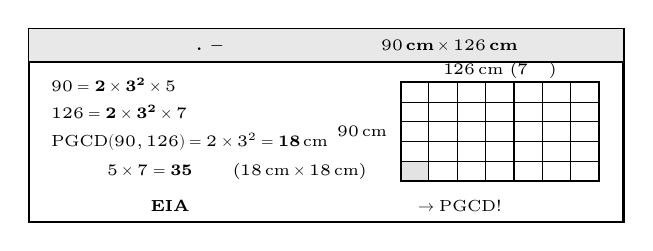
\begin{tikzpicture}[x=1cm, y=1cm, every node/.style={font=\fontsize{5.8pt}{7.6pt}\selectfont, text=black}]
  \draw[black, line width=0.9pt] (0,0) rectangle (7.55,2.45);
  \fill[gray!18] (0,2.03) rectangle (7.55,2.45);
  \draw[black, line width=0.6pt] (0,2.03) -- (7.55,2.03);
  \node at (3.775,2.24) {\textbf{លំហាត់គំរូ ទំ.២១–២២៖ ក្រាលឥដ្ឋការ៉ូការេលើបន្ទប់ទឹក $90\unit{cm} \times 126\unit{cm}$}};

  % Left calculation
  \node[anchor=west] at (0.16,1.74) {$90 = \mathbf{2 \times 3^2} \times 5$};
  \node[anchor=west] at (0.16,1.40) {$126 = \mathbf{2 \times 3^2} \times 7$};
  \node[anchor=west] at (0.16,1.02) {$\operatorname{PGCD}(90,126) = 2\times 3^2 = \mathbf{18\unit{cm}}$};
  \node[anchor=west] at (0.16,0.64) {ចំនួនការ៉ូ៖ $5 \times 7 = \mathbf{35}$ សន្លឹក ($18\unit{cm}\times 18\unit{cm}$)};

  % Right 5x7 grid matching textbook p.22
  \begin{scope}[shift={(4.72,0.52)}]
    \fill[gray!22] (0,0) rectangle (0.36,0.25);
    \draw[black, line width=0.75pt] (0,0) rectangle (2.52,1.25);
    \foreach \i in {1,...,6} {
      \draw[black, line width=0.4pt] (\i*0.36,0) -- (\i*0.36,1.25);
    }
    \foreach \j in {1,...,4} {
      \draw[black, line width=0.4pt] (0,\j*0.25) -- (2.52,\j*0.25);
    }
    \node at (1.26,1.40) {$126\unit{cm}$ ($7$ ជួរ)};
    \node[anchor=east] at (-0.05,0.625) {$90\unit{cm}$};
  \end{scope}

  \node at (3.775,0.20) {\textbf{\en{EIA}៖} បំបែកចតុកោណកែងជាការេប៉ុនៗគ្នាធំបំផុតដោយគ្មានសល់ $\to \operatorname{PGCD}$!};
\end{tikzpicture}}

% ៣ខ. E5 Practice: ប្រតិបត្តិ ទំ.២២ (ចែកសៀវភៅ 24 ក្បាល និងខ្មៅដៃ 36 ដើម)
\newcommand{\figPracticeDIVTwoFive}{%
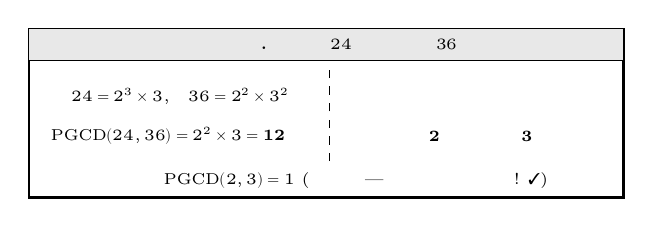
\begin{tikzpicture}[x=1cm, y=1cm, every node/.style={font=\fontsize{5.7pt}{7.5pt}\selectfont, text=black}]
  \draw[black, line width=0.9pt] (0,0) rectangle (7.55,2.14);
  \fill[gray!18] (0,1.74) rectangle (7.55,2.14);
  \draw[black, line width=0.6pt] (0,1.74) -- (7.55,1.74);
  \node at (3.775,1.94) {\textbf{លំហាត់ប្រតិបត្តិ ទំ.២២៖ ចែកសៀវភៅ $24$ ក្បាល និងខ្មៅដៃ $36$ ដើម}};
  \node at (1.92,1.28) {$24 = 2^3 \times 3,\quad 36 = 2^2 \times 3^2$};
  \node at (1.92,0.78) {$\operatorname{PGCD}(24,36) = 2^2\times 3 = \mathbf{12}$ នាក់};
  \draw[black, dashed, line width=0.5pt] (3.82,0.46) -- (3.82,1.64);
  \node at (5.68,1.28) {សិស្សម្នាក់ៗទទួលបាន៖};
  \node at (5.68,0.78) {សៀវភៅ $\mathbf{2}$ ក្បាល និងខ្មៅដៃ $\mathbf{3}$ ដើម};
  \node at (3.775,0.22) {ផ្ទៀងផ្ទាត់៖ $\operatorname{PGCD}(2, 3) = 1$ (បឋមរវាងគ្នា — ពិតជាចំនួនសិស្សច្រើនបំផុតមែន! \ding{51})};
\end{tikzpicture}}

% ៤. E5 Evaluate: សំណួរវិនិច្ឆ័យ A-D លើ A = 2^3 x 3^2 x 5 និង B = 2^2 x 3^4 x 7
\newcommand{\figExitDIVTwoFive}{%
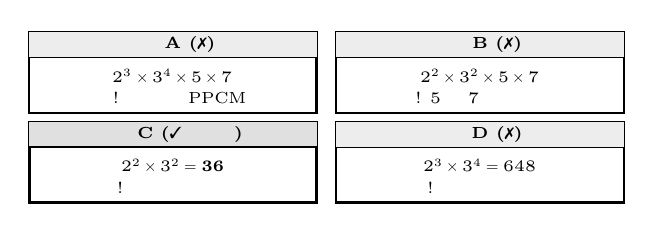
\begin{tikzpicture}[x=1cm, y=1cm, every node/.style={font=\fontsize{5.8pt}{7.5pt}\selectfont, text=black}]
  % Choice A
  \draw[black, line width=0.8pt] (0,1.14) rectangle (3.65,2.16);
  \fill[gray!14] (0,1.84) rectangle (3.65,2.16);
  \draw[black, line width=0.5pt] (0,1.84) -- (3.65,1.84);
  \node at (1.825,2.00) {\textbf{ជម្រើស \en{A} (\ding{55})}};
  \node at (1.825,1.61) {$2^3 \times 3^4 \times 5 \times 7$};
  \node at (1.825,1.33) {ខុស! នេះជាក្បួនរក $\operatorname{PPCM}$};

  % Choice B
  \draw[black, line width=0.8pt] (3.90,1.14) rectangle (7.55,2.16);
  \fill[gray!14] (3.90,1.84) rectangle (7.55,2.16);
  \draw[black, line width=0.5pt] (3.90,1.84) -- (7.55,1.84);
  \node at (5.725,2.00) {\textbf{ជម្រើស \en{B} (\ding{55})}};
  \node at (5.725,1.61) {$2^2 \times 3^2 \times 5 \times 7$};
  \node at (5.725,1.33) {ខុស! $5$ និង $7$ មិនមែនកត្តារួមទេ};

  % Choice C (Correct)
  \draw[black, line width=1.05pt] (0,0) rectangle (3.65,1.02);
  \fill[gray!24] (0,0.70) rectangle (3.65,1.02);
  \draw[black, line width=0.6pt] (0,0.70) -- (3.65,0.70);
  \node at (1.825,0.86) {\textbf{ជម្រើស \en{C} (\ding{51} ត្រឹមត្រូវ)}};
  \node at (1.825,0.47) {$2^2 \times 3^2 = \mathbf{36}$};
  \node at (1.825,0.19) {ត្រូវ! កត្តារួម និទស្សន្តតូចជាងគេ};

  % Choice D
  \draw[black, line width=0.8pt] (3.90,0) rectangle (7.55,1.02);
  \fill[gray!14] (3.90,0.70) rectangle (7.55,1.02);
  \draw[black, line width=0.5pt] (3.90,0.70) -- (7.55,0.70);
  \node at (5.725,0.86) {\textbf{ជម្រើស \en{D} (\ding{55})}};
  \node at (5.725,0.47) {$2^3 \times 3^4 = 648$};
  \node at (5.725,0.19) {ខុស! ច្រឡំយកនិទស្សន្តធំជាងគេ};
\end{tikzpicture}}

\begin{document}
\fontsize{10pt}{15.2pt}\selectfont

% ============================================================================
% ក្បាលរដ្ឋបាល (Administrative Header — តាមគំរូ ls_plan.tex)
% ============================================================================
{\centering
  {\muol\fontsize{11pt}{16pt}\selectfont ព្រះរាជាណាចក្រកម្ពុជា\par}
  {\muol\fontsize{11pt}{16pt}\selectfont ជាតិ សាសនា ព្រះមហាក្សត្រ\par}
  \vspace{-3pt}{\khmflourish\par}
}

\vspace{1pt}
{\muol\fontsize{10pt}{15.5pt}\selectfont
មន្ទីរអប់រំ យុវជន និងកីឡា ខេត្តកំពង់ធំ\par
ការិយាល័យអប់រំ យុវជន និងកីឡា ស្រុកកំពង់ស្វាយ\par
អនុវិទ្យាល័យព្រះក្រសាំង\par}

\vspace{2pt}
{\centering{\muol\fontsize{11.5pt}{17pt}\selectfont កិច្ចតែងការបង្រៀន\par}}
\vspace{2pt}

% --- ព័ត៌មានទូទៅ ---
{\hspace*{2.8cm}\renewcommand{\arraystretch}{1.08}
\begin{tabular}{@{}l@{\hspace{0.35cm}}p{2.9cm}@{\hspace{0.15cm}}c@{\hspace{0.25cm}}l@{}}
  - & មុខវិជ្ជា & : & គណិតវិទ្យា ថ្នាក់ទី៧ (ពីជគណិត) \\
  - & ចំណងជើងមេរៀន & : & មេរៀនទី២៖ តួចែកនិងពហុគុណ \\
  - & ចំណងជើងរង & : & ៥. តួចែករួមធំបំផុត (\en{PGCD} ឬ \en{GCD}) (ទំ.២១--២២) \\
  - & រយៈពេល & : & ១ ម៉ោងសិក្សា (៥០ នាទី) \\
  - & បង្រៀនដោយ & : & ហុក ប៊ុនថែន \\
  - & កាលបរិច្ឆេទ & : & ថ្ងៃអង្គារ ទី១៧ ខែវិច្ឆិកា ឆ្នាំ២០២៦ \\
\end{tabular}\par}

\vspace{2pt}

% --- I. វត្ថុបំណង ---
{\muol\fontsize{10pt}{15.5pt}\selectfont \enbf{I.} វត្ថុបំណង\par}
\vspace{1pt}
{\renewcommand{\arraystretch}{1.10}
\begin{tabular}{@{}p{0.55cm}@{}p{2.35cm}@{\hspace{0.15cm}}c@{\hspace{0.25cm}}p{14.95cm}@{}}
  \hfill\wcirc\hspace{0.2cm} & វិជ្ជាសម្បទា & : & សិស្សប្រាប់បានពីនិយមន័យនិងវិធានរកតួចែករួមធំបំផុត (\en{PGCD}) ព្រមទាំងអត្ថន័យនៃពីរចំនួនបឋមរវាងគ្នាបានត្រឹមត្រូវ (ទំ.២១) ។ \\
  \hfill\wcirc\hspace{0.2cm} & បំណិនសម្បទា & : & សិស្សគណនា \en{PGCD} នៃពីរឬច្រើនចំនួនតាមផលគុណកត្តាបឋម និងដោះស្រាយចំណោទចែកស្មើ/ក្រាលការេលើសន្លឹកកិច្ចការបានត្រឹមត្រូវ ។ \\
  \hfill\wcirc\hspace{0.2cm} & ចរិយាសម្បទា & : & សិស្សមានទម្លាប់ពិនិត្យភាពចែកដាច់ឡើងវិញ មិនចាញ់បោកពាក្យ «ធំបំផុត» និងចេះសហការចែករំលែកដោយស្មើភាពក្នុងក្រុម ។ \\
\end{tabular}\par}

\vspace{2pt}

% --- II. សម្ភារៈឧបទេស ---
{\muol\fontsize{10pt}{15.5pt}\selectfont \enbf{II.} សម្ភារៈឧបទេស\par}
\vspace{1pt}
\hspace*{0.55cm}$\bullet$\ សៀវភៅសិក្សាគោលថ្នាក់ទី៧ (ទំ.២១--២២ និងទំ.២៤) ក្ដារខៀន ដីស/ហ្វឺត និង\textbf{សន្លឹកកិច្ចការសិស្សបំពេញចន្លោះ ស-ខ្មៅ} (កូដ \en{DIV25} ទំព័រ ១--២ សម្រាប់សិស្ស និងទំព័រ ៣ ប្លង់ក្ដារខៀន/ចម្លើយគ្រូ — គ្មានប្រើ \en{LCD})\par

\vspace{2pt}

% --- III. វិធីសាស្រ្តបង្រៀន ---
{\muol\fontsize{10pt}{15.5pt}\selectfont \enbf{III.} វិធីសាស្រ្តបង្រៀន\par}
\vspace{1pt}
{\renewcommand{\arraystretch}{1.08}
\begin{tabular}{@{}p{0.55cm}@{}p{2.35cm}@{\hspace{0.15cm}}c@{\hspace{0.25cm}}p{14.95cm}@{}}
  \hfill$\bullet$\hspace{0.2cm} & គោលវិធី & : & សិស្សមជ្ឈមណ្ឌល (សន្លឹកកិច្ចការបំពេញចន្លោះជាគោល + ការពិភាក្សាជាក្រុមតូច ៣ នាក់) \\
  \hfill$\bullet$\hspace{0.2cm} & យុទ្ធវិធីបង្រៀន & : & គំរូស្ថាបនានិយម \en{5Es} រួមបញ្ចូល \textbf{តារាងតម្រឹមជួរឈរកត្តាបឋម និងចម្រាញ់និទស្សន្តតូចជាងគេ (\en{Prime-Column Alignment})} \\
\end{tabular}\par}

\vspace{2pt}

% --- IV. ដំណើរការបង្រៀន ---
{\muol\fontsize{10pt}{15.5pt}\selectfont \enbf{IV.} ដំណើរការបង្រៀន\par}

{\renewcommand{\arraystretch}{1.14}
\begin{longtable}{|L{5.50cm}|L{7.90cm}|L{4.80cm}|}
\hline
\multicolumn{1}{|c|}{\cellcolor{headgray}\muol សកម្មភាពគ្រូ} &
\multicolumn{1}{c|}{\cellcolor{headgray}\muol ខ្លឹមសារមេរៀន} &
\multicolumn{1}{c|}{\cellcolor{headgray}\muol សកម្មភាពសិស្ស} \\
\hline
\endfirsthead

\hline
\multicolumn{1}{|c|}{\cellcolor{headgray}\muol សកម្មភាពគ្រូ} &
\multicolumn{1}{c|}{\cellcolor{headgray}\muol ខ្លឹមសារមេរៀន} &
\multicolumn{1}{c|}{\cellcolor{headgray}\muol សកម្មភាពសិស្ស} \\
\hline
\endhead

% ==================== ជំហានទី១ (2min) ====================
\stepheader{ជំហានទី១ \enbf{(}រដ្ឋបាលថ្នាក់\enbf{)}}
$\bullet$ ពិនិត្យវត្តមាន អនាម័យ និងសណ្ដាប់ធ្នាប់ថ្នាក់រៀន \par
$\bullet$ រៀបចំក្រុមតូច ៣ នាក់តាមតុ និងចែក\textbf{សន្លឹកកិច្ចការសិស្ស (\en{DIV25} ទំព័រ ១–២)}
&
$\bullet$ រដ្ឋបាលថ្នាក់ អនាម័យ និងវិន័យសិក្សា \par
$\bullet$ ចែកសន្លឹកកិច្ចការម្នាក់ ១ សន្លឹក សម្រាប់បំពេញតាមដំណាក់កាល \en{E1--E5}
&
$\circ$ ប្រធានថ្នាក់រាយការណ៍វត្តមានសិស្ស \par
$\circ$ ទទួលសន្លឹកកិច្ចការ សរសេរឈ្មោះ និងអង្គុយតាមក្រុម ៣ នាក់ \\
\hline

% ==================== ជំហានទី២ (9min: កំណែ <=3m + រំលឹក 3m + E1 3m) ====================
\stepheader{ជំហានទី២ \enbf{(}កិច្ចការផ្ទះ \enbf{+} ទំនាក់ទំនងមេរៀនថ្មី\enbf{)}}
\ditem \textbf{កំណែកិច្ចការផ្ទះ ($\le\text{\enbf{3\,min}}$)} \par
$\bullet$ ហៅសិស្សផ្ទៀងផ្ទាត់ចម្លើយលំហាត់ទំ.២៤ លេខ ៥ លើក្ដារខៀនឆ្វេង
&
{\centering\redsub{កំណែកិច្ចការផ្ទះមេរៀនមុន (ទំ.២៤ លេខ ៥)}\par}
$\bullet$ $63=3^2\times 7,\ 100=2^2\times 5^2,\ 129=3\times 43,\ 225=3^2\times 5^2$ \par
$\bullet$ $567=3^4\times 7,\ 1\,980=2^2\times 3^2\times 5\times 11,\ 2\,097=3^2\times 233$ \par
$\bullet$ $50\,336=2^5\times 11^2\times 13,\quad 127\,008=2^5\times 3^4\times 7^2$
&
$\circ$ ផ្ទៀងចម្លើយលេខ ៥ និងកែចូលសៀវភៅ \\[3pt]

\ditem \textbf{រំលឹកមេរៀនទាក់ទង (\enbf{3min})} \par
$\bullet$ សួរ៖ «ចូរបំបែក $12$ និង $18$ ជាផលគុណកត្តាបឋម និងរកតួចែកនៃ $12$!»
&
{\centering\redsub{រំលឹកផលគុណកត្តាបឋម និងបញ្ជីតួចែក}\par}
$\bullet$ $12 = \mathbf{2^2 \times 3}$ \quad និង \quad $18 = \mathbf{2 \times 3^2}$ \par
$\bullet$ តួចែកនៃ $12$ គឺ៖ $\{1, 2, 3, 4, 6, 12\}$
&
$\circ$ ឆ្លើយបំបែក $12=2^2\times 3,\ 18=2\times 3^2$ និងរាយតួចែក \\[3pt]

\fiveE{E1 - Engage (3min)} \timenote{(កុំទាន់ផ្ដល់ចម្លើយ)} \par
\ditem \textbf{បេសកកម្មអន្ទាក់ពាក្យ «ធំបំផុត» ក្នុង $\operatorname{PGCD}(12, 18)$ (\en{E1})}
&
\redsub{បេសកកម្ម \en{E1}៖ តើអ្នកណារកតួចែករួមធំបំផុតនៃ $12$ និង $18$ ត្រូវ?}
&
$\circ$ អានស្ថានភាពបញ្ហា \en{E1} \\[3pt]

$\bullet$ ឱ្យសិស្សពិភាក្សាជាគូលើសន្លឹកកិច្ចការ \en{E1} រវាងសិស្ស ក ($36$) និងសិស្ស ខ ($6$)
&
$\bullet$ \textbf{សិស្ស ក៖} «ព្រោះរកតួចែករួម\textbf{ធំបំផុត} ត្រូវយកនិទស្សន្តធំ៖ $2^2\times 3^2 = 36$!» \par
$\bullet$ \textbf{សិស្ស ខ៖} «$12$ ចែកមិនដាច់នឹង $36$ ទេ! ត្រូវយកនិទស្សន្តតូច៖ $2\times 3 = 6$!»
&
$\circ$ ពិភាក្សាជាគូ និងគូស \ding{51} ក្នុងប្រអប់ \en{E1} \\[3pt]

&
\cfig{\figEngageDIVTwoFive}
& \\
\hline

% ==================== ជំហានទី៣ (17min: E2 11m + E3 6m) ====================
\stepheader{ជំហានទី៣ \enbf{(}ខ្លឹមសារមេរៀនថ្មី\enbf{)}}
\fiveE{E2 - Explore (11min)} \par
$\bullet$ សរសេរចំណងជើងរង \textbf{៥. តួចែករួមធំបំផុត (\en{PGCD} ឬ \en{GCD})} \par
\ditem \textbf{សកម្មភាព ១៖ ប្រៀបធៀប ២ វិធីលើ $30$ និង $36$ (ឧទាហរណ៍ 1 ទំ.២១, \enbf{5.5min})}
&
៥. តួចែករួមធំបំផុត (\en{PGCD} ឬ \en{GCD}) (ទំ.២១) \par
$\bullet$ \textbf{ឧទាហរណ៍ 1 (រក $\operatorname{PGCD}$ នៃ $30$ និង $36$)៖} \par
\hspace*{0.15cm}-- \textbf{វិធីទី 1 (បញ្ជីតួចែក)៖} តួចែកនៃ $30$: $\{1, 2, 3, 5, 6, 10, 15, 30\}$; តួចែកនៃ $36$: $\{1, 2, 3, 4, 6, 9, 12, 18, 36\} \implies$ តួចែករួម៖ $1, 2, 3, 6 \implies \operatorname{PGCD}(30,36) = \mathbf{6}$
&
$\circ$ រាយតួចែក រកតួចែករួម និងឃើញ $\operatorname{PGCD}(30,36)=6$ លើ \en{E2-A} \\[3pt]

$\bullet$ ឱ្យសិស្សតម្រឹមជួរឈរកត្តាបឋមនៃ $30$ និង $36$ ក្នុងប្រអប់លើ \en{E2-A} (ទំ.២១)
&
\hspace*{0.15cm}-- \textbf{វិធីទី 2 (កត្តាបឋម)៖} $30 = 2 \times 3 \times 5$ និង $36 = 2^2 \times 3^2$ \par
គូសប្រអប់ជួរឈរកត្តារួម ($2$ និង $3$) យកនិទស្សន្តតូចជាងគេ៖ $\operatorname{PGCD}(30, 36) = 2 \times 3 = \mathbf{6}$
&
$\circ$ គូសប្រអប់ជួរឈរកត្តារួម ឃើញបាន $2\times 3=6$ ដូចគ្នា! \\[3pt]

\ditem \textbf{សកម្មភាព ២៖ ចំនួនបីតួ និងចំនួនបឋមរវាងគ្នា (ឧទាហរណ៍ 2–3 ទំ.២១, \enbf{5.5min})} \par
$\bullet$ ឱ្យសិស្សបំពេញប្រអប់ជួរឈររក $\operatorname{PGCD}(60, 180, 210)$ និងពិនិត្យចំនួនបឋមរវាងគ្នា
&
$\bullet$ \textbf{ឧទាហរណ៍ 2៖} $60 = 2^2\times 3\times 5$, $180 = 2^2\times 3^2\times 5$, $210 = 2\times 3\times 5\times 7$ \par
$\implies \operatorname{PGCD}(60, 180, 210) = 2 \times 3 \times 5 = \mathbf{30}$ \par
$\bullet$ \textbf{ឧទាហរណ៍ 3 (បឋមរវាងគ្នា)៖} $\operatorname{PGCD}(11, 13) = \mathbf{1}$ និង $\operatorname{PGCD}(8, 15) = \mathbf{1}$
&
$\circ$ បំពេញប្រអប់ជួរឈររកឃើញ $30$ និងសង្កេត $\operatorname{PGCD}(8,15)=1$ \\[3pt]

&
\cfig{\figPrimeColsDIVTwoFive}
& \\[3pt]

% --- E3 Explain (6min) ---
\fiveE{E3 - Explain (6min)} \par
$\bullet$ ដឹកនាំសិស្សសង្ខេបប្រអប់ «ជាទូទៅ» (ទំ.២១) លើសន្លឹកកិច្ចការ \en{E3}
&
$\bullet$ \textbf{ជាទូទៅ (ទំ.២១)៖} ដើម្បីរកតួចែករួមធំបំផុតនៃពីរ ឬច្រើនចំនួន គេបំបែកចំនួននីមួយៗជាផលគុណកត្តាបឋម រួចគេគុណ\graybox{កត្តារួមទាំងអស់ដែលមាននិទស្សន្តតូចជាងគេ} ។
&
$\circ$ បំពេញប្រអប់វិធានទូទៅលើ \en{E3} \\[3pt]

$\bullet$ សង្ខេប «សម្គាល់» អំពីចំនួនបឋមរវាងគ្នា (ទំ.២១)
&
$\bullet$ \textbf{សម្គាល់ (ទំ.២១)៖} ពីរចំនួន\textbf{បឋមរវាងគ្នា} កាលណា $\operatorname{PGCD}$ របស់វាស្មើនឹង $\graybox{$1$}$ (ឧ. $8$ និង $15$ ជាចំនួនបឋមរវាងគ្នា ទោះវាមិនមែនជាចំនួនបឋមក៏ដោយ) ។
&
$\circ$ កត់សម្គាល់និយមន័យចំនួនបឋមរវាងគ្នា \\[3pt]

$\bullet$ ភ្ជាប់\textbf{ធនាគារហេតុផល \cnum{1}--\cnum{2}} លើក្ដារខៀន និងសន្លឹកកិច្ចការ
&
\textbf{ធនាគារហេតុផល (\en{Warrant Bank})៖} \par
\cnum{1} \textbf{លក្ខខណ្ឌតួចែករួម៖} $\operatorname{PGCD}(a,b)$ ត្រូវចែកដាច់ទាំង $a$ និង $b$ ($\operatorname{PGCD} \le \min(a,b)$) \par
\cnum{2} \textbf{ជ្រើសតែកត្តារួម៖} ជ្រើសតែកត្តាបឋមដែលមានក្នុង\textbf{គ្រប់ចំនួនទាំងអស់} (ផាត់ចោលកត្តាមិនរួម)
&
$\circ$ ផ្ទៀងលេខកូដ \cnum{1}--\cnum{2} លើសន្លឹកកិច្ចការ \\[3pt]

$\bullet$ ភ្ជាប់\textbf{ធនាគារហេតុផល \cnum{3}--\cnum{4}} សម្រាប់និទស្សន្តតូច និងបឋមរវាងគ្នា
&
\cnum{3} \textbf{និទស្សន្តតូចជាងគេ៖} ក្នុងជួរឈរកត្តារួមនីមួយៗ ជ្រើសយក\textbf{និទស្សន្តតូចជាងគេ} រួចគុណគ្នា \par
\cnum{4} \textbf{បឋមរវាងគ្នា៖} បើគ្មានកត្តាបឋមរួមសោះ នោះ $\operatorname{PGCD} = 1$ (ហាមសរសេរស្មើ $0$!)
&
$\circ$ ផ្ទៀងលេខកូដ \cnum{3}--\cnum{4} លើសន្លឹកកិច្ចការ \\
\hline

% ==================== ជំហានទី៤ (20min: E4 10m + E5 10m) ====================
\stepheader{ជំហានទី៤ \enbf{(}ពង្រីកចំណេះដឹង\enbf{)}}
\fiveE{E4 - Elaborate (10min)} \par
\ditem \textbf{លំហាត់គំរូតាមសៀវភៅគោល ទំ.២១–២២ (ក្រាលការ៉ូបន្ទប់ទឹក $90\unit{cm}\times 126\unit{cm}$)}
&
{\muol លំហាត់គំរូ} \textbf{(សៀវភៅគោល ទំ.២១–២២ — ក្រាលឥដ្ឋការ៉ូការេធំបំផុត)៖} \par
$\bullet$ បន្ទប់ទឹករាងចតុកោណកែងមានទទឹង $90\unit{cm}$ និងបណ្ដោយ $126\unit{cm}$ ។
&
$\circ$ អានប្រធានលំហាត់គំរូ និងកត់សម្គាល់ទំហំ $90\unit{cm}\times 126\unit{cm}$ \\[3pt]

$\bullet$ ដឹកនាំសិស្សបកស្រាយហេតុផលប្រើ $\operatorname{PGCD}$ និងបំបែក $90,\ 126$ លើ \en{E4}
&
$\bullet$ \textbf{១) រកប្រវែងជ្រុងការ៉ូ៖} ដើម្បីក្រាលការេពេញដោយមិនកាត់ និងមានផ្ទៃធំបំផុត ជ្រុងការេត្រូវស្មើ $\operatorname{PGCD}(90, 126)$ (\cnum{1})៖ \par
ដោយ $90 = 2\times 3^2\times 5$ និង $126 = 2\times 3^2\times 7 \implies \operatorname{PGCD}(90,126) = 2\times 3^2 = \graybox{$18\unit{cm}$}$ (\cnum{2}, \cnum{3})
&
$\circ$ បំបែក $90$ និង $126$ រកឃើញជ្រុងការ៉ូ $18\unit{cm}$ \\[3pt]

$\bullet$ ឱ្យសិស្សគណនាចំនួនការ៉ូសរុបដែលត្រូវប្រើតាមទទឹង និងបណ្ដោយ
&
$\bullet$ \textbf{២) រកចំនួនការ៉ូ៖} តាមទទឹង $90\div 18 = 5$ ជួរ និងតាមបណ្ដោយ $126\div 18 = 7$ ជួរ \par
ដូចនេះ ចំនួនការ៉ូសរុបគឺ៖ $5 \times 7 = \graybox{$35$ សន្លឹក}$ ។
&
$\circ$ គណនាឃើញចំនួនការ៉ូ $5\times 7 = 35$ សន្លឹក \\[3pt]

&
\cfig{\figTilesDIVTwoFive}
& \\[3pt]

$\bullet$ សួរសំណួរឆ្លុះបញ្ចាំង \textbf{\en{EIA Looking-Back} (1min)} សម្គាល់ពាក្យគន្លឹះចំណោទ $\operatorname{PGCD}$
&
\textbf{\en{EIA Looking-Back}៖} «តើសញ្ញាសម្គាល់អ្វីឱ្យដឹងថាចំណោទត្រូវប្រើ $\operatorname{PGCD}$?» ($\to$ គឺការ\textbf{កាត់បំបែក ឬចែកស្មើៗគ្នា}ជាចំណែក/ការេធំបំផុតដោយគ្មានសល់!)
&
$\circ$ កត់ចំណាំសញ្ញាសម្គាល់ចំណោទ $\operatorname{PGCD}$ \\[3pt]

% --- E5 Evaluate (10min) ---
\fiveE{E5 - Evaluate (10min)} \par
\ditem \textbf{ប្រតិបត្តិជាក្រុមតូច ៣ នាក់ (4min, សន្លឹកកិច្ចការ \en{E5})} \par
$\bullet$ ឱ្យក្រុមសិស្សដោះស្រាយប្រតិបត្តិទំ.២២៖ ចែកសៀវភៅ $24$ ក្បាល និងខ្មៅដៃ $36$ ដើម
&
{\muol លំហាត់ប្រតិបត្តិ} \textbf{(សៀវភៅគោល ទំ.២២ — ចែកសៀវភៅ $24$ និងខ្មៅដៃ $36$)៖} \par
$\bullet$ បំបែក៖ $24 = 2^3 \times 3$ និង $36 = 2^2 \times 3^2$ \par
$\bullet$ ចំនួនសិស្សច្រើនបំផុត៖ $\operatorname{PGCD}(24, 36) = 2^2 \times 3 = \mathbf{12}$ \textbf{នាក់} (\cnum{2}, \cnum{3})
&
$\circ$ សហការគ្នាដោះស្រាយឃើញចែកឱ្យសិស្សបាន $12$ នាក់ \\[3pt]

&
\cfig{\figPracticeDIVTwoFive}
& \\[3pt]

$\bullet$ ឱ្យក្រុមសិស្សបញ្ជាក់ចំណែកម្នាក់ៗ និង\textbf{បិទបេសកកម្ម \en{E1} (2min)}
&
$\bullet$ ម្នាក់ៗបាន៖ សៀវភៅ $24\div 12 = 2$ ក្បាល និងខ្មៅដៃ $36\div 12 = 3$ ដើម \par
$\bullet$ \textbf{បិទបេសកកម្ម \en{E1}៖} \textbf{សិស្ស ខ} ត្រឹមត្រូវ! $\operatorname{PGCD}(12, 18) = 2\times 3 = \mathbf{6}$ (\cnum{1}, \cnum{3}) ។
&
$\circ$ បិទបេសកកម្ម \en{E1} ឃើញសិស្ស ខ ត្រឹមត្រូវ \\[3pt]

\ditem \textbf{សំណួរវិនិច្ឆ័យ \en{A--D} និងសំបុត្រចេញ (4min)} \par
$\bullet$ សរសេរជម្រើស \en{A--D} លើក្ដារខៀន សម្រាប់ $A=2^3\times 3^2\times 5$ និង $B=2^2\times 3^4\times 7$
&
{\centering\textbf{សំណួរវិនិច្ឆ័យ \en{A--D}៖ តើ $\operatorname{PGCD}(A, B)$ ស្មើនឹងមួយណា?}\par}
&
$\circ$ ពិនិត្យជម្រើសទាំង ៤ តាមកូដហេតុផល \cnum{2}--\cnum{3} \\[3pt]

$\bullet$ ឱ្យសិស្សគូសរង្វង់លើសន្លឹកកិច្ចការ និងលើកម្រាមដៃ ១--៤ ព្រមគ្នា
&
$\bullet$ ផាត់ចោល \en{A, B} (មានកត្តាមិនរួម $5, 7$) និង \en{D} (យកនិទស្សន្តធំ $2^3\times 3^4$) \par
$\bullet$ \textbf{ជម្រើស \en{C} ត្រឹមត្រូវ៖} យកកត្តារួម $2, 3$ និទស្សន្តតូចជាងគេបាន $2^2\times 3^2 = \mathbf{36}$!
&
$\circ$ គូសរង្វង់លើសន្លឹកកិច្ចការ និងលើកម្រាមដៃ ៣ (\textbf{ជម្រើស \en{C}}) \\[3pt]

&
\cfig{\figExitDIVTwoFive}
& \\[3pt]

$\bullet$ បញ្ជាក់ចម្លើយត្រូវ (\textbf{ជម្រើស \en{C}}) និងឱ្យបំពេញ\textbf{សំបុត្រចេញ ៦០ វិនាទី}
&
$\bullet$ \textbf{សំបុត្រចេញ៖} រក $\operatorname{PGCD}(45, 75)$ ($45=3^2\times 5,\ 75=3\times 5^2 \implies \mathbf{15}$) ។
&
$\circ$ គណនា $\operatorname{PGCD}(45, 75) = 15$ មុនបញ្ចប់ម៉ោង \\
\hline

% ==================== ជំហានទី៥ (<=2min) ====================
\stepheader{ជំហានទី៥ \enbf{(}កិច្ចការផ្ទះ \enbf{+} បណ្ដាំផ្ញើ\enbf{)}}
\timenote{ចំណាយពេលឱ្យតិចបំផុតកុំឱ្យលើស 2min} \par
$\bullet$ ណែនាំប្រអប់\textbf{កិច្ចការផ្ទះ}លើសន្លឹកកិច្ចការទំព័រ ២ (សៀវភៅគោល ទំ.២៤ លេខ ៦, ៨, ១០)
&
{\centering{\muol កិច្ចការផ្ទះ} \textbf{(សៀវភៅគោល ទំ.២៤ លេខ ៦, លេខ ៨ និង លេខ ១០)}\par} \par
$\bullet$ \textbf{លេខ ៦៖} រក $\operatorname{PGCD}$ នៃ៖ ក. $9, 15$; ខ. $10, 108$; គ. $128, 324$; ឃ. $192, 160, 96$; ង. $48, 72, 132$; ច. $36, 168, 144, 252$ ។
&
$\circ$ គូសចំណាំលំហាត់ទំ.២៤ លេខ ៦, ៨, ១០ \\[3pt]

$\bullet$ បញ្ជាក់ប្រធានលេខ ៨ និងលេខ ១០ ព្រមទាំងផ្ដាំផ្ញើអានចំណុច ៦ (\en{PPCM})
&
$\bullet$ \textbf{លេខ ៨៖} រក $x, y$ ($0<x<y$) បើ $\operatorname{PGCD}(x,y)=12$ និង $x+y=72$ ។ \textbf{លេខ ១០៖} កាត់ក្រណាត់ $24\unit{cm}\times 56\unit{cm}$ ធ្វើកូនកន្សែងដៃការេធំបំផុត ។ \par
$\bullet$ \textbf{បណ្ដាំផ្ញើ៖} អានមុន \textbf{៦. ពហុគុណរួមតូចបំផុត (\en{PPCM})} (សៀវភៅគោល ទំ.២២–២៣) ។
&
$\circ$ កត់ត្រាបណ្ដាំផ្ញើ ទុកសន្លឹកកិច្ចការក្នុងសៀវភៅ និងជម្រាបលាគ្រូ \\
\hline
\end{longtable}}

\vspace{6pt}
% --- ហត្ថលេខា (កាលបរិច្ឆេទត្រូវគ្នា ១០០% នឹងខាងលើ) ---
{\centering
\hspace*{5.2cm}\begin{minipage}{11.5cm}
  \centering
  ថ្ងៃអង្គារ ៨កើត ខែកត្តិក ឆ្នាំមមី អដ្ឋស័ក ពុទ្ធសករាជ ២៥៧០\par
  កំពង់ស្វាយ, ថ្ងៃទី១៧ ខែវិច្ឆិកា ឆ្នាំ២០២៦\par
  \vspace{2pt}
  {\muol គ្រូបង្រៀន\par}
  \vspace{32pt}
  \hfill{\muol ហុក ប៊ុនថែន}\hspace*{1.4cm}
\end{minipage}\par}

\end{document}
